\section{Trabalhos Correlatos}

Muitos autores gostam de apontar como algumas linguaguens de programação são mais eficientes que outras 
quando testadas sobre alguns parâmetros.
No artigo \citetitle{C++vsPython} de \citeauthor{C++vsPython}, mostra-se como a diferença na escolha das ferramentas
usadas durante a construção de um \emph{software} tem grandes impactos no desempenho final de uma aplicação como
mostrado na figura \ref{fig:comparisonMemorycppvspython}.

\begin{figure}[!ht]
    \centering
    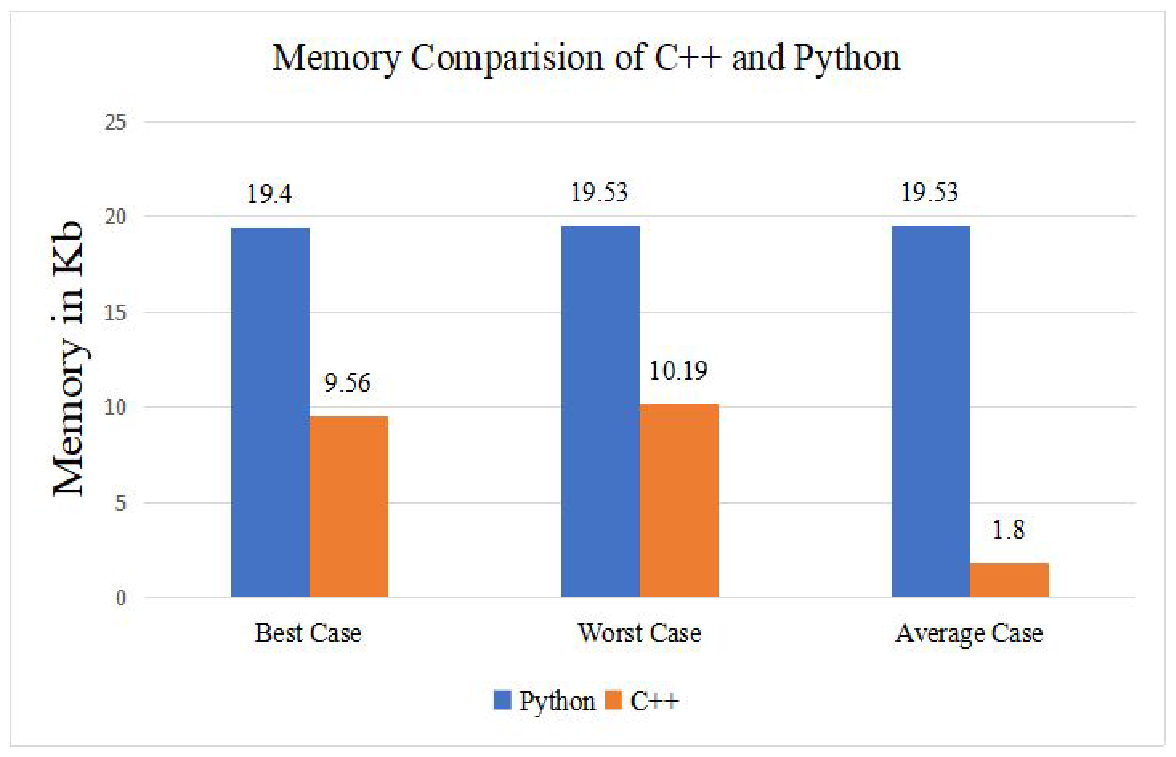
\includegraphics[width=0.5\textwidth]{ComparisonofMemoryConsumptionofSearchingAlgorithm.png}
    \caption[a]{Comparação do uso de memória em um algoritmo de busca\footnotemark.}
    \label{fig:comparisonMemorycppvspython}
\end{figure}

\footnotetext{Retirado do artigo: \citetitle{C++vsPython}.}

O uso de memória é extremamente importante de ser pensado quando se trata de um contexto de treinamento
de IA. O tempo de execução também é de suma importância de ser calculado, uma vez que teremos sempre 
grandes entradas para trabalhar. Pode-se ver na figura \ref{fig:speedcppvspython} a diferença de performance
entre ambas as línguas.

\begin{figure}[!ht]
    \centering
    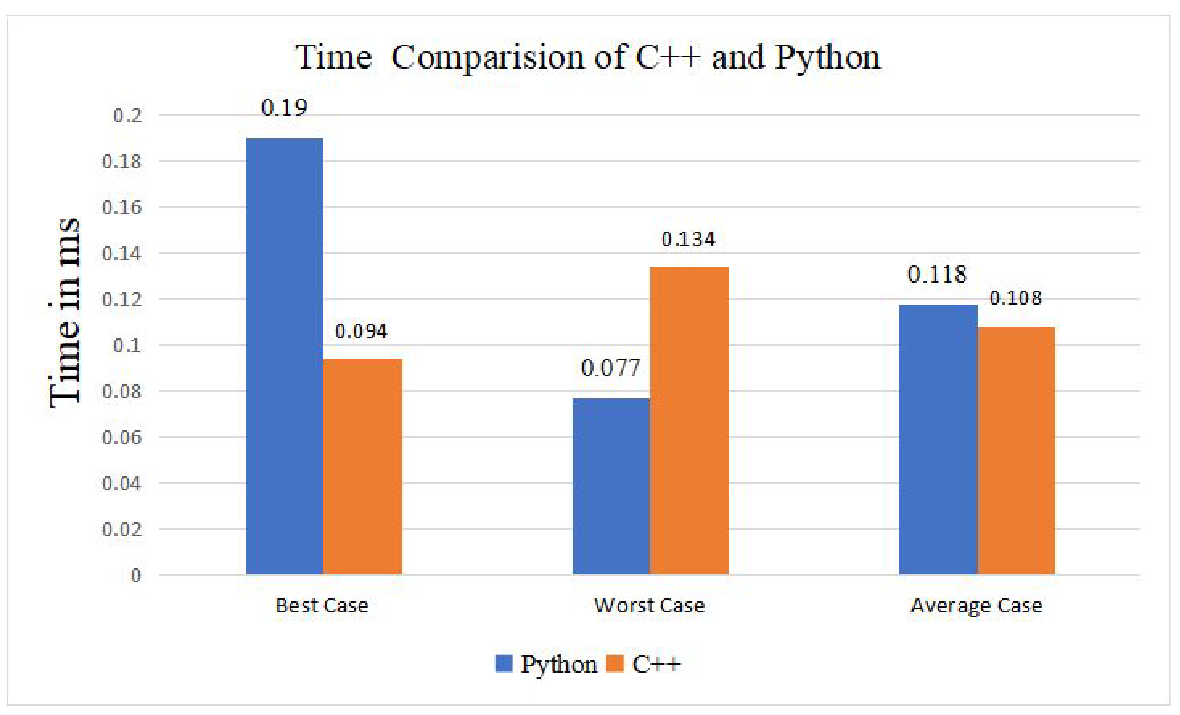
\includegraphics[width=0.5\textwidth]{ComparisonofTimeUtilizationofSearchingAlgorithm.png}
    \caption[a]{Comparação do tempo de execução de um algoritmo de busca de forma sequencial\footnotemark.}
    \label{fig:speedcppvspython}
\end{figure}

\footnotetext{Retirado do artigo: \citetitle{C++vsPython}.}

É notório que a linguagem de programação Python ficou atrás da linguagem C++ nesses parâmetros medidos. 
A primeira é consideravelmente mais simples de usar e ensinar para novos programadores \cite{C++vsPython}. 
Com isso em mente, o pesquisador \citeauthor{HPC_Python} apresentou em seu artigo \citetitle{HPC_Python},
como Python se tornou a língua favorita para os professores ensinarem e sua imensa utilidade na área científica. 
Por conta de sua facilidade de uso, houve grande atenção da comunidade para aumentar o desempenho dessa língua, até
que fique competitiva com o C++.

Trabalhos foram feitos para aumentar sua eficiência como citado por \citeauthor{JIT}, que em seu trabalho
para a IBM já em 2007, pensava em como aumentar o desempenho da linguagem de programação Java usando 
\emph{Just-in-Time Compiler}. Esse recurso permite que uma língua seja compilada para \emph{Bytecode}, o que
seria equivalente a uma lingua de programação intermediária entre o que a máquina consegue entender e o que o 
programador efetivamente escreveu. Isso permitia que um código não fosse completamente compilado para uma arquitetura
específica de processador, mas no momento de sua execução fosse modificado para o código de montagem de máquina
mais eficiente que estivesse disponível \cite{JIT}.

Considerando que Python é uma linguagem interpretada. Unir a ideia do \emph{JIT} que estava sendo empregada a 
vários anos no interpretador de Python poderia gerar bons resultados. O primeiro teste feito por \citeauthor{NumbaLLVMJIT}
apresentou ótimos resultados como mostrado na figura \ref{fig:numbavspythonsequencial}.

\begin{figure}[ht]
    \centering
    \begin{tabular}{|c|c|c|}
        \hline
        Tamanho da Matriz & Numba & C \\
        \hline
        64 x 64 & 463x & 453x \\
        \hline
        128 x 128 & 454x & 407x \\
        \hline 
        256 x 256 & 280x & 263x \\
        \hline
        512 x 512 & 276x & 268x \\
        \hline
    \end{tabular}
    \caption[a]{Comparativo entre o tempo de execução do Numba e de um código em C para multiplicação de matrizes\footnotemark[3].}
    \label{fig:numbavspythonsequencial}
\end{figure}

% Aparece no final da página, não está relacionado com o texto que está sendo escrito em volta
\footnotetext[3]{Retirado do artigo: \citetitle{NumbaLLVMJIT}.}

Com esses resultados é possível comprovar que com as otimizações certas, pode-se tornar o Python tão performático quanto C++.
Muitas outras otimizações foram feitas para ter-se ainda mais desempenho como \emph{deferred loop specialization}, reescrita
das equações das matrizes e o uso de ferramentas para geração de \emph{Bytecode} otimizados com LLVM.

Algoritmos para seleção de melhor instância como o \emph{K-Means} sempre foram referência quando discute-se
sobre algoritmos de \emph{clusterização}. No artigo escrito por \citeauthor{KmeansAlgorithm} \cite{KmeansAlgorithm},
mostra-se como há várias implementações extremamente eficientes para esse algoritmo e como a ordem de complexidade
pode ser elevada, assim como mostrado na figura \ref{fig:complexitykmeans}.

\begin{figure}[ht]
    \centering
    \begin{tabular}{|c|c|c|c|}
        \hline
        Complexidade & \emph{K-Means} & \emph{Constrained-K-Means} & \emph{X-Means} \\
        \hline 
        Tempo & $O(n^2)$ & $O(kn)$ & $O(n\log k_{max})$ \\
        \hline  
        Espaço & $O((n+k)d)$ & $O((n+k)d)$ & $O((n+k)d)$ \\
        \hline
    \end{tabular}
    \caption[a]{Complexidade de algumas implementações do \emph{K-Means}\footnotemark.}
    \label{fig:complexitykmeans}
\end{figure}

\footnotetext{Retirado do artigo: \citetitle{KmeansAlgorithm}.}

Neste artigo será usado \emph{CUDA} para otimizar o algoritmo \emph{Ant Colony Optimization} usando a biblioteca
\emph{CuPy} \cite{Cupy} que permite o uso de cálculos de matrizes em GPUs Nvidia. Essa biblioteca
tem como objetivo acelerar o processamento de arranjos multidimensionais, com isso torna-se perfeita
para todos os algoritmos já citados neste artigo.

Será usado o \emph{K-Means} como unidade comparativa deste trabalho para mensurar 
o ganho que a \emph{Ant Colony Optimization} é capaz de obter, tanto quanto sua acertividade
em encontrar o melhor caminho. Aproveitando de todas as otimizações que já foram citadas previamente
e todos os trabalhos que foram feitos para tornar o Python a ferramenta mais procurada
para pesquisadores de inteligências artificiais. Com isso, esse trabalho tem como objetivo
avançar as pesquisas previamente feitas para testar a eficácia de uma versão otimizada em 
GPU do algoritmo ACO.
